\documentclass[xcolor=table]{beamer}

\usepackage[utf8]{inputenc}
\usepackage[latin1]{inputenc}
\usepackage[francais]{babel}
\usepackage[T1]{fontenc}

\usepackage{verbatim}
\usepackage{pifont}
\usepackage{eso-pic}
\usepackage{pgf}

\usetheme{Rochester}
%\usetheme{Boadilla}
\setbeamertemplate{footline}
{
  \leavevmode%
  \hbox{%
  \begin{beamercolorbox}[wd=.333333\paperwidth,ht=2.25ex,dp=1ex,center]{author in head/foot}%
    \usebeamerfont{author in head/foot}\insertshortauthor
  \end{beamercolorbox}%
  \begin{beamercolorbox}[wd=.333333\paperwidth,ht=2.25ex,dp=1ex,center]{title in head/foot}%
    \usebeamerfont{title in head/foot}\insertshorttitle
  \end{beamercolorbox}%
  \begin{beamercolorbox}[wd=.333333\paperwidth,ht=2.25ex,dp=1ex,right]{date in head/foot}%
    \usebeamerfont{date in head/foot}\insertshortdate{}\hspace*{2em}
    \insertframenumber{} / \inserttotalframenumber\hspace*{2ex} 
  \end{beamercolorbox}}%
  \vskip0pt%
}
\usecolortheme{seahorse}

\setbeamertemplate{navigation symbols}{} 

\title[PSAR 12 : Kilobot]{\Huge{Kilobot}}
\subtitle{Impl\'ementation d'algorithmes pour les cohortes de robots}
\author[Benjamin Bielle, Arnaud Guermont]{Benjamin Bielle\\Arnaud Guermont}

\institute{Universit\'e Pierre et Marie Curie}
\date{12 mai 2015}

%\logo{
\includegraphics[height=0.5cm]{upmc.png}}
\titlegraphic{%
\includegraphics[width=2cm]{upmc.png}\hspace*{4.75cm}~%
   
\includegraphics[width=2cm]{upmc.png}
}

\begin{document}

%%%%%%%%%%%%%%
% PAGE TITRE %
%%%%%%%%%%%%%%
\begin{frame}
  \titlepage
\end{frame}

\begin{frame}
  \frametitle{Vue d'ensemble} % Table of contents slide, comment this block out to remove it
  \tableofcontents % Throughout your presentation, if you choose to use \section{} and \subsection{} commands, these will automatically be printed on this slide as an overview of your presentation
\end{frame}

%%%%%%%%%%%%%%%%%%%%%%%%%%%%%%%
% SPECIFICATIONS DES KILOBOTS %
%%%%%%%%%%%%%%%%%%%%%%%%%%%%%%%
\section{Sp\'ecifications des kilobots}
\begin{frame}
  \frametitle{Sp\'ecifications des kilobots}
  La plate-forme Kilobot est définie par les caractéristiques suivantes : 
  \begin{columns}[T] % align columns
    \begin{column}{.48\textwidth}
      %% Left Part
      \begin{figure}[!h]
        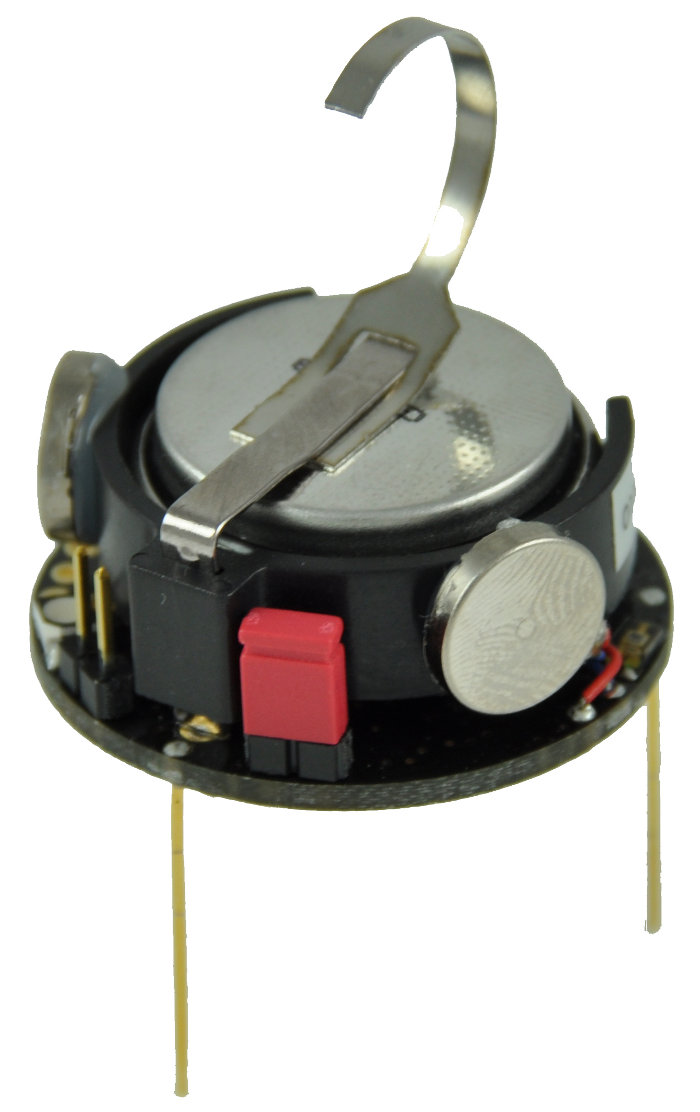
\includegraphics[width=3cm]{kilobotSpecs.jpg}
      \end{figure}
    \end{column}%
    \hfill%
    \begin{column}{.48\textwidth}
      %%  Right Part
      \begin{itemize}
        \item Communication par infrarouge
        \item D\'eplacement par vibration
        \item Mesure de la lumi\`ere ambiante
        \item Essaim contr\^olable par un seul op\'erateur
        \item Faible co\^ut de fabrication
      \end{itemize}
    \end{column}%
  \end{columns}
\end{frame}

%%%%%%%%%%%%%%%
% SIMULATEURS %
%%%%%%%%%%%%%%%
\section{Simulateurs}
\begin{frame}
  \frametitle{Simulateurs}
  \begin{columns}[T] % align columns
    \begin{column}{.48\textwidth}
      %% Left Part
      \Large V-Rep
      \setbeamerfont*{itemize/enumerate body}{size=\footnotesize}
      \begin{itemize}
        \item[\ding{51}] Polyvalent
        \item[\ding{51}] Programmation par scripts LUA
        \item[\ding{51}] Moteur physique avanc\'e
        \item[\ding{55}] Ne supporte pas la mise \`a l'\'echelle
      \end{itemize}
      \begin{figure}[!h]
        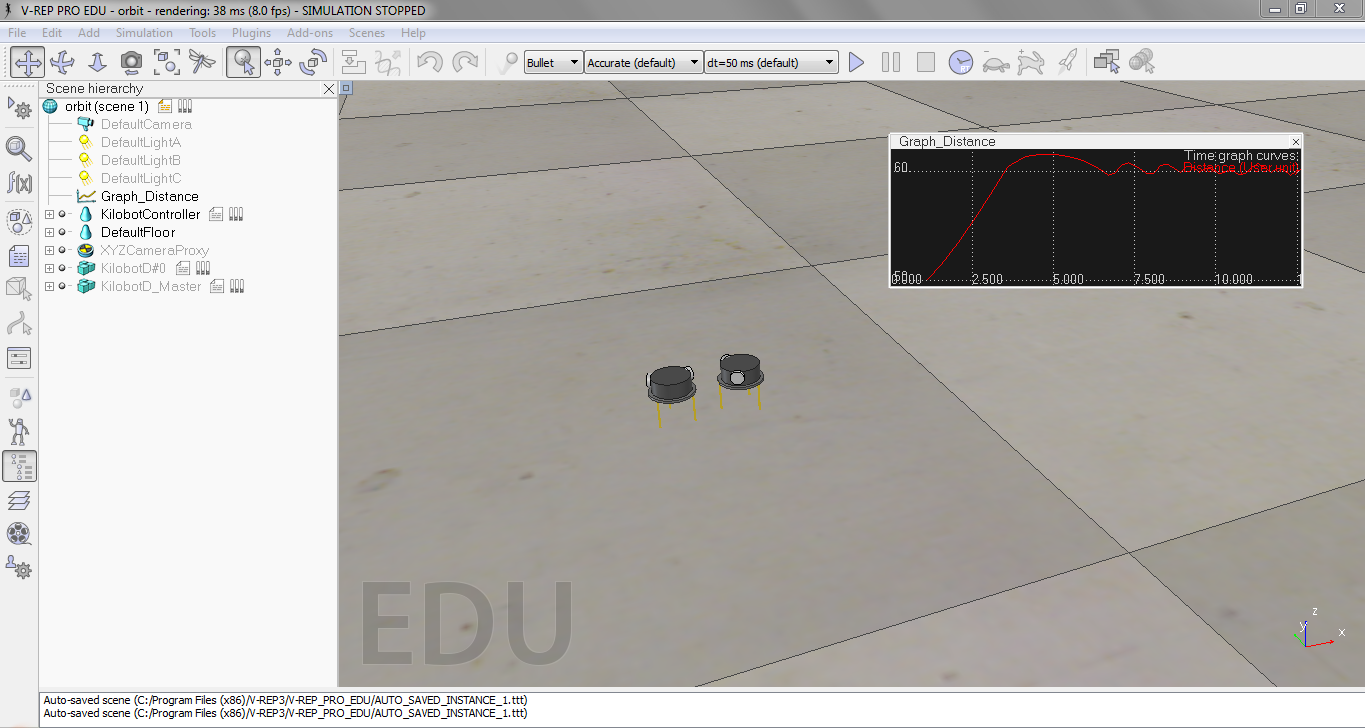
\includegraphics[width=5cm]{V-Rep.png}
      \end{figure}
    \end{column}%
    \hfill%
    \begin{column}{.48\textwidth}
      %%  Right Part
      \Large KbSim
      \setbeamerfont*{itemize/enumerate body}{size=\footnotesize}
      \begin{itemize}
        \item[\ding{51}] Simulateur d\'edi\'e
        \item[\ding{51}] Programmation Python
        \item[\ding{51}] L\'eger
        \item[\ding{51}] Simulation d'un grand nombre de kilobots
      \end{itemize}
      \begin{figure}[!h]
        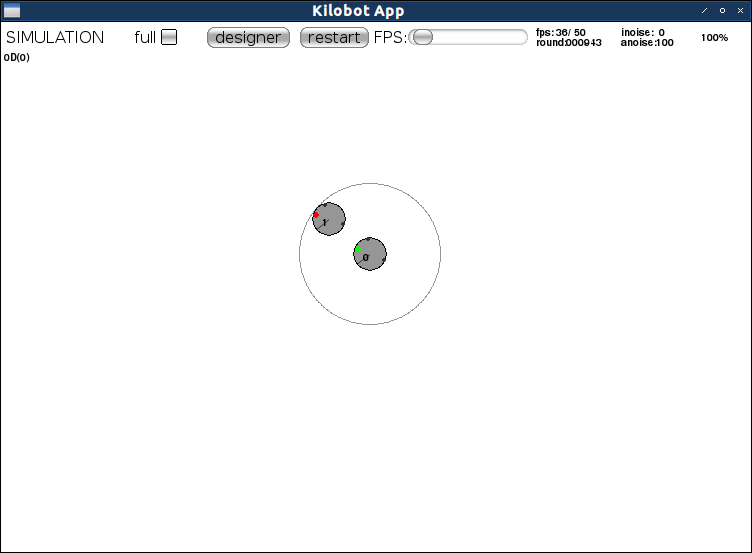
\includegraphics[width=4cm]{KbSim.png}
      \end{figure}
    \end{column}%
  \end{columns}
\end{frame}

%%%%%%%%%%%
% PHASE I %
%%%%%%%%%%%
\section{Phase I}
\begin{frame}
  \frametitle{Phase I}
  \begin{center}
    \Huge \textbf{Phase I}
  \end{center}
  \begin{block}{Objectifs}
    \begin{itemize}
      \setbeamertemplate{itemize item}[triangle]
      \item Recherche documentaire
      \item Prise en main
    \end{itemize}
  \end{block}
\end{frame}

%%%%%%%%%%%%
% FIRMWARE %
%%%%%%%%%%%%

\begin{frame}
  \frametitle{Phase I}
  \framesubtitle{Firmware}
  Caractéristiques des firmwares disponibles :\\
  \begin{center}
    \rowcolors{1}{white!20}{white!10} 
    \begin{tabular}{l!{\vrule}cccc} 
      & K-Team & Kilobotics \\ \hline 
      Compatible linux   & \color{red}\ding{55}     & \color{green}\ding{51} \\ 
      Open source        & \color{red}\ding{55}   & \color{green}\ding{51}   \\ 
      Fonctions avancées & \color{red}\ding{55}   & \color{green}\ding{51}   \\
    \end{tabular}
  \end{center}
  \begin{block}{Flashage}
    Flashages des kilobots et du contrôleur via l'outil AVRDUDE
  \end{block}
\end{frame}

%%%%%%%%%%%%%%%%%
% PRISE EN MAIN %
%%%%%%%%%%%%%%%%%
\begin{frame}[fragile]
  \frametitle{Phase I}
  \framesubtitle{Prise en main}
  \begin{block}{Algorithme de l'orbite}
    Un robot dessine une orbite autour d'un autre et maintient sa distance de message
  \end{block}
  \bigskip
  \begin{block}{Algorithme de synchronisation}
    Chaque robot envoie son horloge et l'ajuste en fonction des messages re\c cus
  \end{block}
\end{frame}

%%%%%%%%%%%%
% PHASE II %
%%%%%%%%%%%%
\section{Phase II}
\begin{frame}
  \frametitle{Phase II}
  \begin{center}
    \Huge \textbf{Phase II}
  \end{center}
  \begin{block}{Objectifs}
    \begin{itemize}
      \setbeamertemplate{itemize item}[triangle]
      \item Implémentation de bio-algorithmes
        \begin{itemize}
        \item Algorithme du phototaxis
        \item Algorithme du gradient
        \end{itemize}
    \end{itemize}
  \end{block}
\end{frame}

%%%%%%%%%%%%%%
% PHOTOTAXIS %
%%%%%%%%%%%%%%
\subsection{Algorithme du phototaxis}
\begin{frame}[fragile]
  \frametitle{Phase II}
  \framesubtitle{Algorithme du phototaxis}
  \begin{block}{Pourquoi ?}
    Propose un bon exemple de comportement de groupe (d'insectes) observé dans la nature
  \end{block}
  \pause
  \begin{block}{Spécifications}
    Chaque robot capte la source lumineuse et ajuste ses déplacements vers celle-ci
  \end{block}
  \pause
  \begin{block}{Contraintes}
    \begin{itemize}
      \setbeamertemplate{itemize item}[triangle]
      \item Environnement à lumière ambiante réduite
      \item Source de lumière dirigée
    \end{itemize}
  \end{block}
\end{frame}

%%%%%%%%%%%%
% GRADIENT %
%%%%%%%%%%%%
\subsection{Algorithme du gradient}
\begin{frame}[fragile]
  \frametitle{Phase II}
  \framesubtitle{Algorithme du gradient}
  \begin{columns}[T] % align columns
    \begin{column}{.48\textwidth}
      %% Left Part
      \bigskip
      \bigskip
      \begin{figure}[!h]
        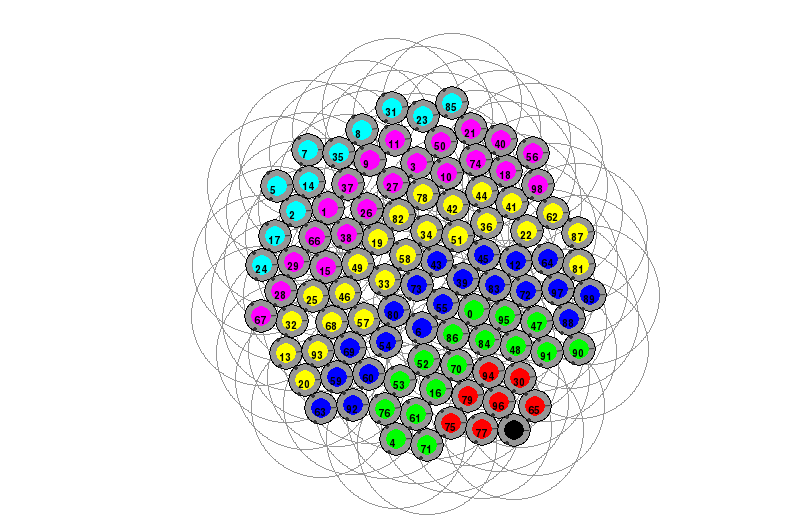
\includegraphics[width=6cm]{gradient.png}
      \end{figure}
    \end{column}%
    \hfill%
    \begin{column}{.48\textwidth}
      %%  Right Part
      \begin{block}{Pourquoi ?}
        Bio-algorithme préambule à la phase III
      \end{block}
      \pause
      \begin{block}{Spécifications}
        Chaque robot calcule la distance qui le sépare de la balise et affiche une couleur en fonction de celle-ci
      \end{block}
      \pause
      \begin{block}{Contraintes}
        Plusieurs robots ont le r\^ole de balise
      \end{block}
    \end{column}
  \end{columns}
\end{frame}

%%%%%%%%%%%%%
% PHASE III %
%%%%%%%%%%%%%
\section{Phase III}
\begin{frame}
  \frametitle{Phase III}
  \begin{center}
    \Huge \textbf{Phase III}
  \end{center}
  \begin{block}{Objectif}
    Implémentation d'un modèle robotique : le modèle \textbf{CORDA}
  \end{block}
  \pause
  \begin{block}{API}
    Réalisation d'une API dont les primitives envisagées sont : \\
    \begin{itemize}
      \setbeamertemplate{itemize item}[triangle]
    \item \textbf{getPosition} qui implémente la seconde approche \pause
    \item \textbf{getVision} qui permet de conna\^itre la position de ses voisins \pause
    \item \textbf{toPosition} qui permet de se rendre à une position donnée
    \end{itemize}
  \end{block}
\end{frame}

%%%%%%%%%
% CORDA %
%%%%%%%%%
\subsection{CORDA}
\begin{frame}
  \frametitle{Phase III}
  \framesubtitle{CORDA}
  \begin{block}{Pourquoi ?}
    Il est largement utilisé pour les algorithmes répartis dans le domaine de la robotique
  \end{block}
  \begin{block}{Description}
    Le modèle CORDA comprend un cycle de 3 phases : Voir, Calculer, Agir
  \end{block}
  \medskip
  \textbf{Contraintes}
  \begin{center}
    \rowcolors{1}{white!20}{white!10} 
    \begin{tabular}{l!{\vrule}cccc} 
      & CORDA & Kilobot \\ \hline 
      Communication     & \color{red}\ding{55}     & \color{green}\ding{51} \\ 
      Vision            & \color{green}\ding{51}   & \color{red}\ding{55}   \\ 
      Repère orthonormé & \color{green}\ding{51}   & \color{red}\ding{55}   \\
      Déplacement précis& \color{green}\ding{51}   & \color{red}\ding{55}
    \end{tabular}
  \end{center}
\end{frame}

%%%%%%%%%%%%%%
% 1 APPROCHE %
%%%%%%%%%%%%%%
\subsection{1\up{ere} Approche}
\begin{frame}
  \frametitle{Phase III}
  \framesubtitle{1\up{ere} Approche}
  \begin{block}{Résultat attendu}
    Localisation des robots
  \end{block}
  \pause
  \begin{block}{Comment ?}
    Utilisation de la triangulation à l'aide de robots fixes ayant le r\^ole de balise
  \end{block}
  \pause
  \begin{block}{Contrainte}
    La distance d'émission des kilobots est limitée à 7cm
  \end{block}
\end{frame}

\begin{frame}
  \frametitle{Phase III}
  \framesubtitle{Résultat obtenu}
  \begin{columns}[T] % align columns
    \begin{column}{.48\textwidth}
      %% Left Part
      \begin{figure}[!h]
        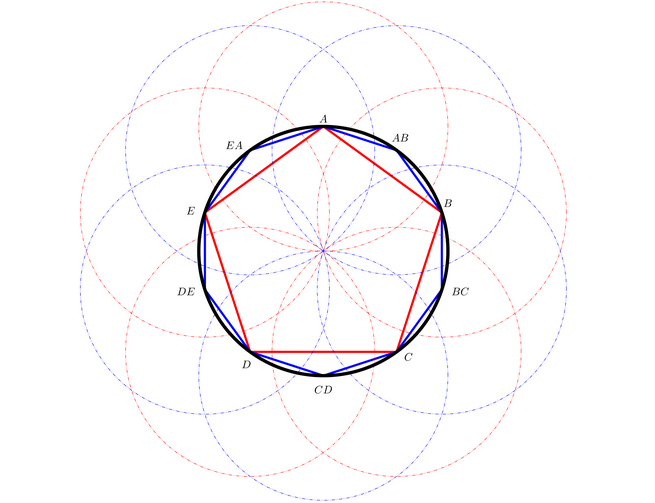
\includegraphics[width=7cm]{Papproche.png}
      \end{figure}
      \pause
    \end{column}%
    \hfill%
    \begin{column}{.58\textwidth}
      %%  Right Part
      \begin{figure}[!h]
        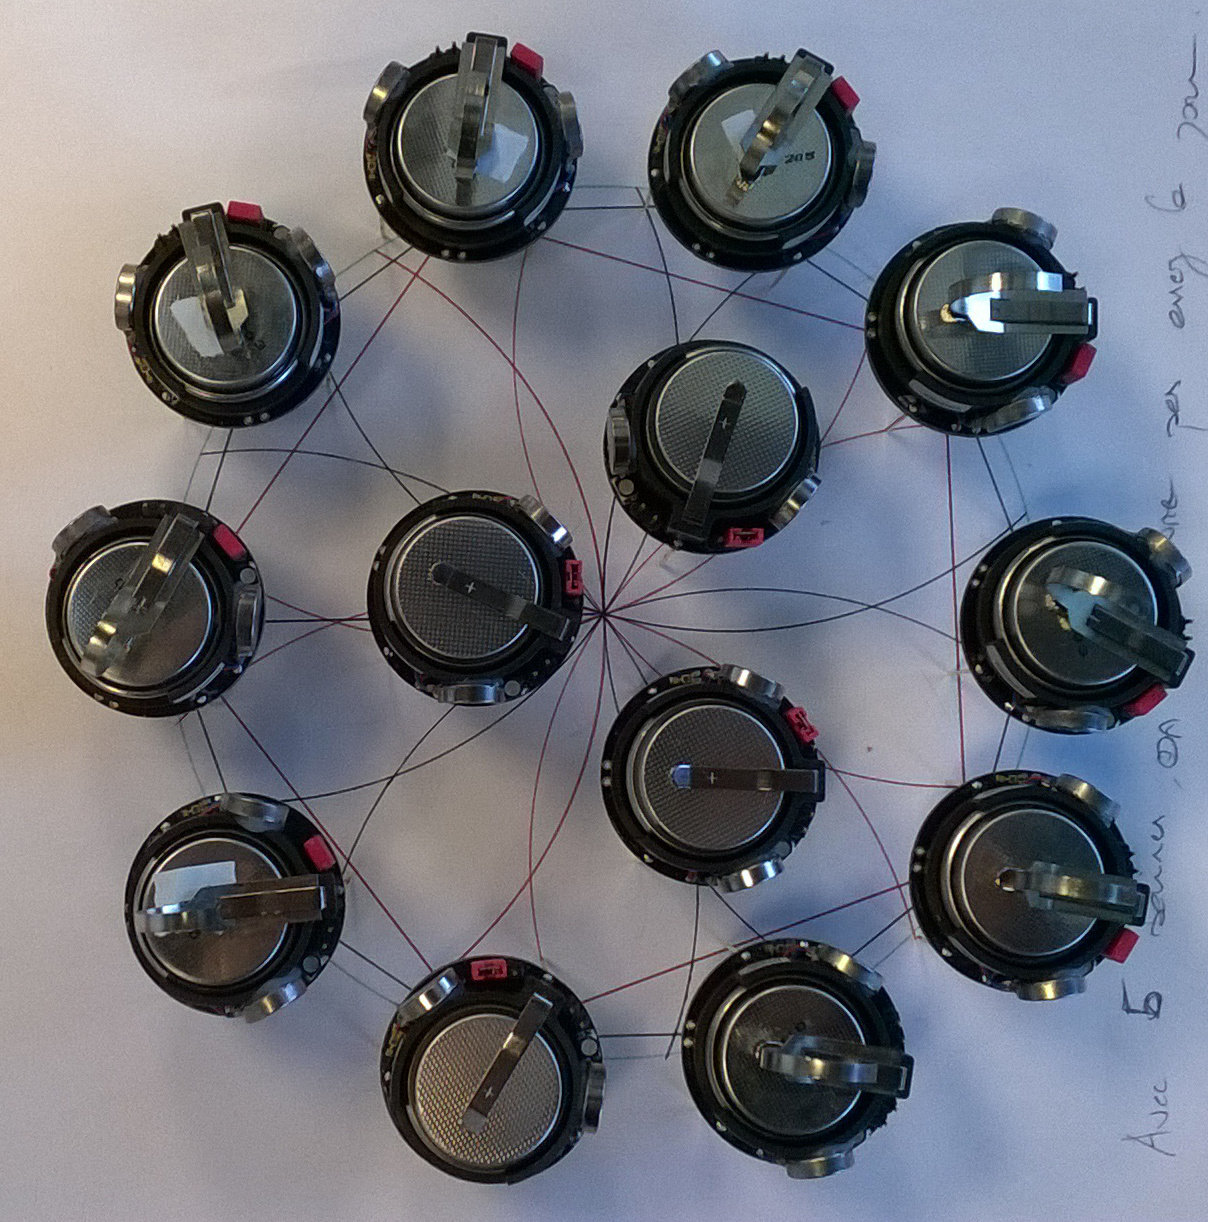
\includegraphics[width=5cm]{locate_bounding_box_demo.jpg}
      \end{figure}
    \end{column}%
  \end{columns}
\end{frame}

%%%%%%%%%%%%%%
% 2 APPROCHE %
%%%%%%%%%%%%%%
\subsection{2\up{e} Approche}
\begin{frame}
  \frametitle{Phase III}
  \framesubtitle{2\up{e} Approche}
  \begin{block}{Résultat attendu}
    Localisation des robots avec un nombre réduit de balises tout en augmentant la portée d'émission
  \end{block}
  \begin{block}{Comment ?}
    Utilisation de la méthode du gradient associée à la méthode vue dans la première approche
  \end{block}
\end{frame}

%%%%%%%%%%%%%%%%%%
% IMPLEMENTATION %
%%%%%%%%%%%%%%%%%%
\subsection{Pistes Expérimentales}
\begin{frame}
  \frametitle{Phase III}
  \framesubtitle{Pistes Expérimentales}
  \begin{block}{Inconvénients}
    \begin{itemize}
      \setbeamertemplate{itemize item}[triangle]
    \item Consommation mémoire pour la détection d'un cycle trop importante \pause
    \item Implémentation des autres primitives menacées par le manque d'espace mémoire \pause
    \item Détection de cycle réparti dynamique
    \end{itemize}
  \end{block}
  \pause
  \begin{figure}[!h]
    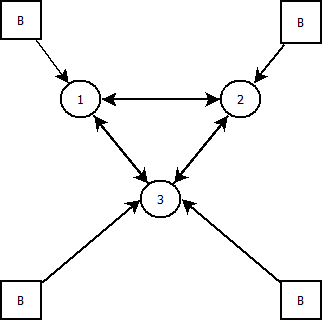
\includegraphics[width=3cm]{schema_cycle.png}
  \end{figure}
\end{frame}

%%%%%%%%%%%%%%%
% CONTRAINTES %
%%%%%%%%%%%%%%%

\subsection{Contraintes}
\begin{frame}
  \frametitle{Contraintes}
  \begin{block}{Solutions}
    Solutions envisageables : \\
    \begin{itemize}
      \setbeamertemplate{itemize item}[triangle]
    \item Implémentation d'une matrice pour la détection des cycles
    \item Utilisation d'un compteur TTL (Time To live)
    \end{itemize}
  \end{block}
  \pause
  \begin{block}{Contraintes}
    Limitations techniques de la plate-forme :\\
    \begin{itemize}
      \setbeamertemplate{itemize item}[triangle]
    \item La matrice occupe trop d'espace mémoire (ne passe pas à l'echelle)
    \item On ne peut pas contrôler les émissions de messages
    \end{itemize}
  \end{block}
\end{frame}

%%%%%%%%%%%%%%
% CONCLUSION %
%%%%%%%%%%%%%%

\subsection{Conclusion}
\begin{frame}
  \frametitle{Conclusion}
  \begin{block}{Objectif}
    Prise en main des kilobots et implémentation du modèle algorithmique CORDA dans la plate-forme
  \end{block}
  \begin{block}{Kilobot}
    \begin{itemize}
      \setbeamertemplate{itemize item}[triangle]
    \item Communication non maîtrisée
    \item D\'eplacement par vibration
    \item Aucun système de positionnement
    \end{itemize}
  \end{block}
  \begin{block}{Conclusion}
    La plate-forme kilobot n'est pas adaptée pour le modèle CORDA
  \end{block}
  Des vidéos sont disponibles sur le github du projet : github.com/LSDev8/PSAR-Kilobot
\end{frame}

\end{document} 
